With respect to the abstract requirements imposed upon project start a brain-storming was performed in order to gather ideas and and identify possible problems in the realization of the project. Figure \ref{mindmap} shows the mind-map resulting from a reflection of these abstract requirements. 
\begin{figure}[h!]
\centering
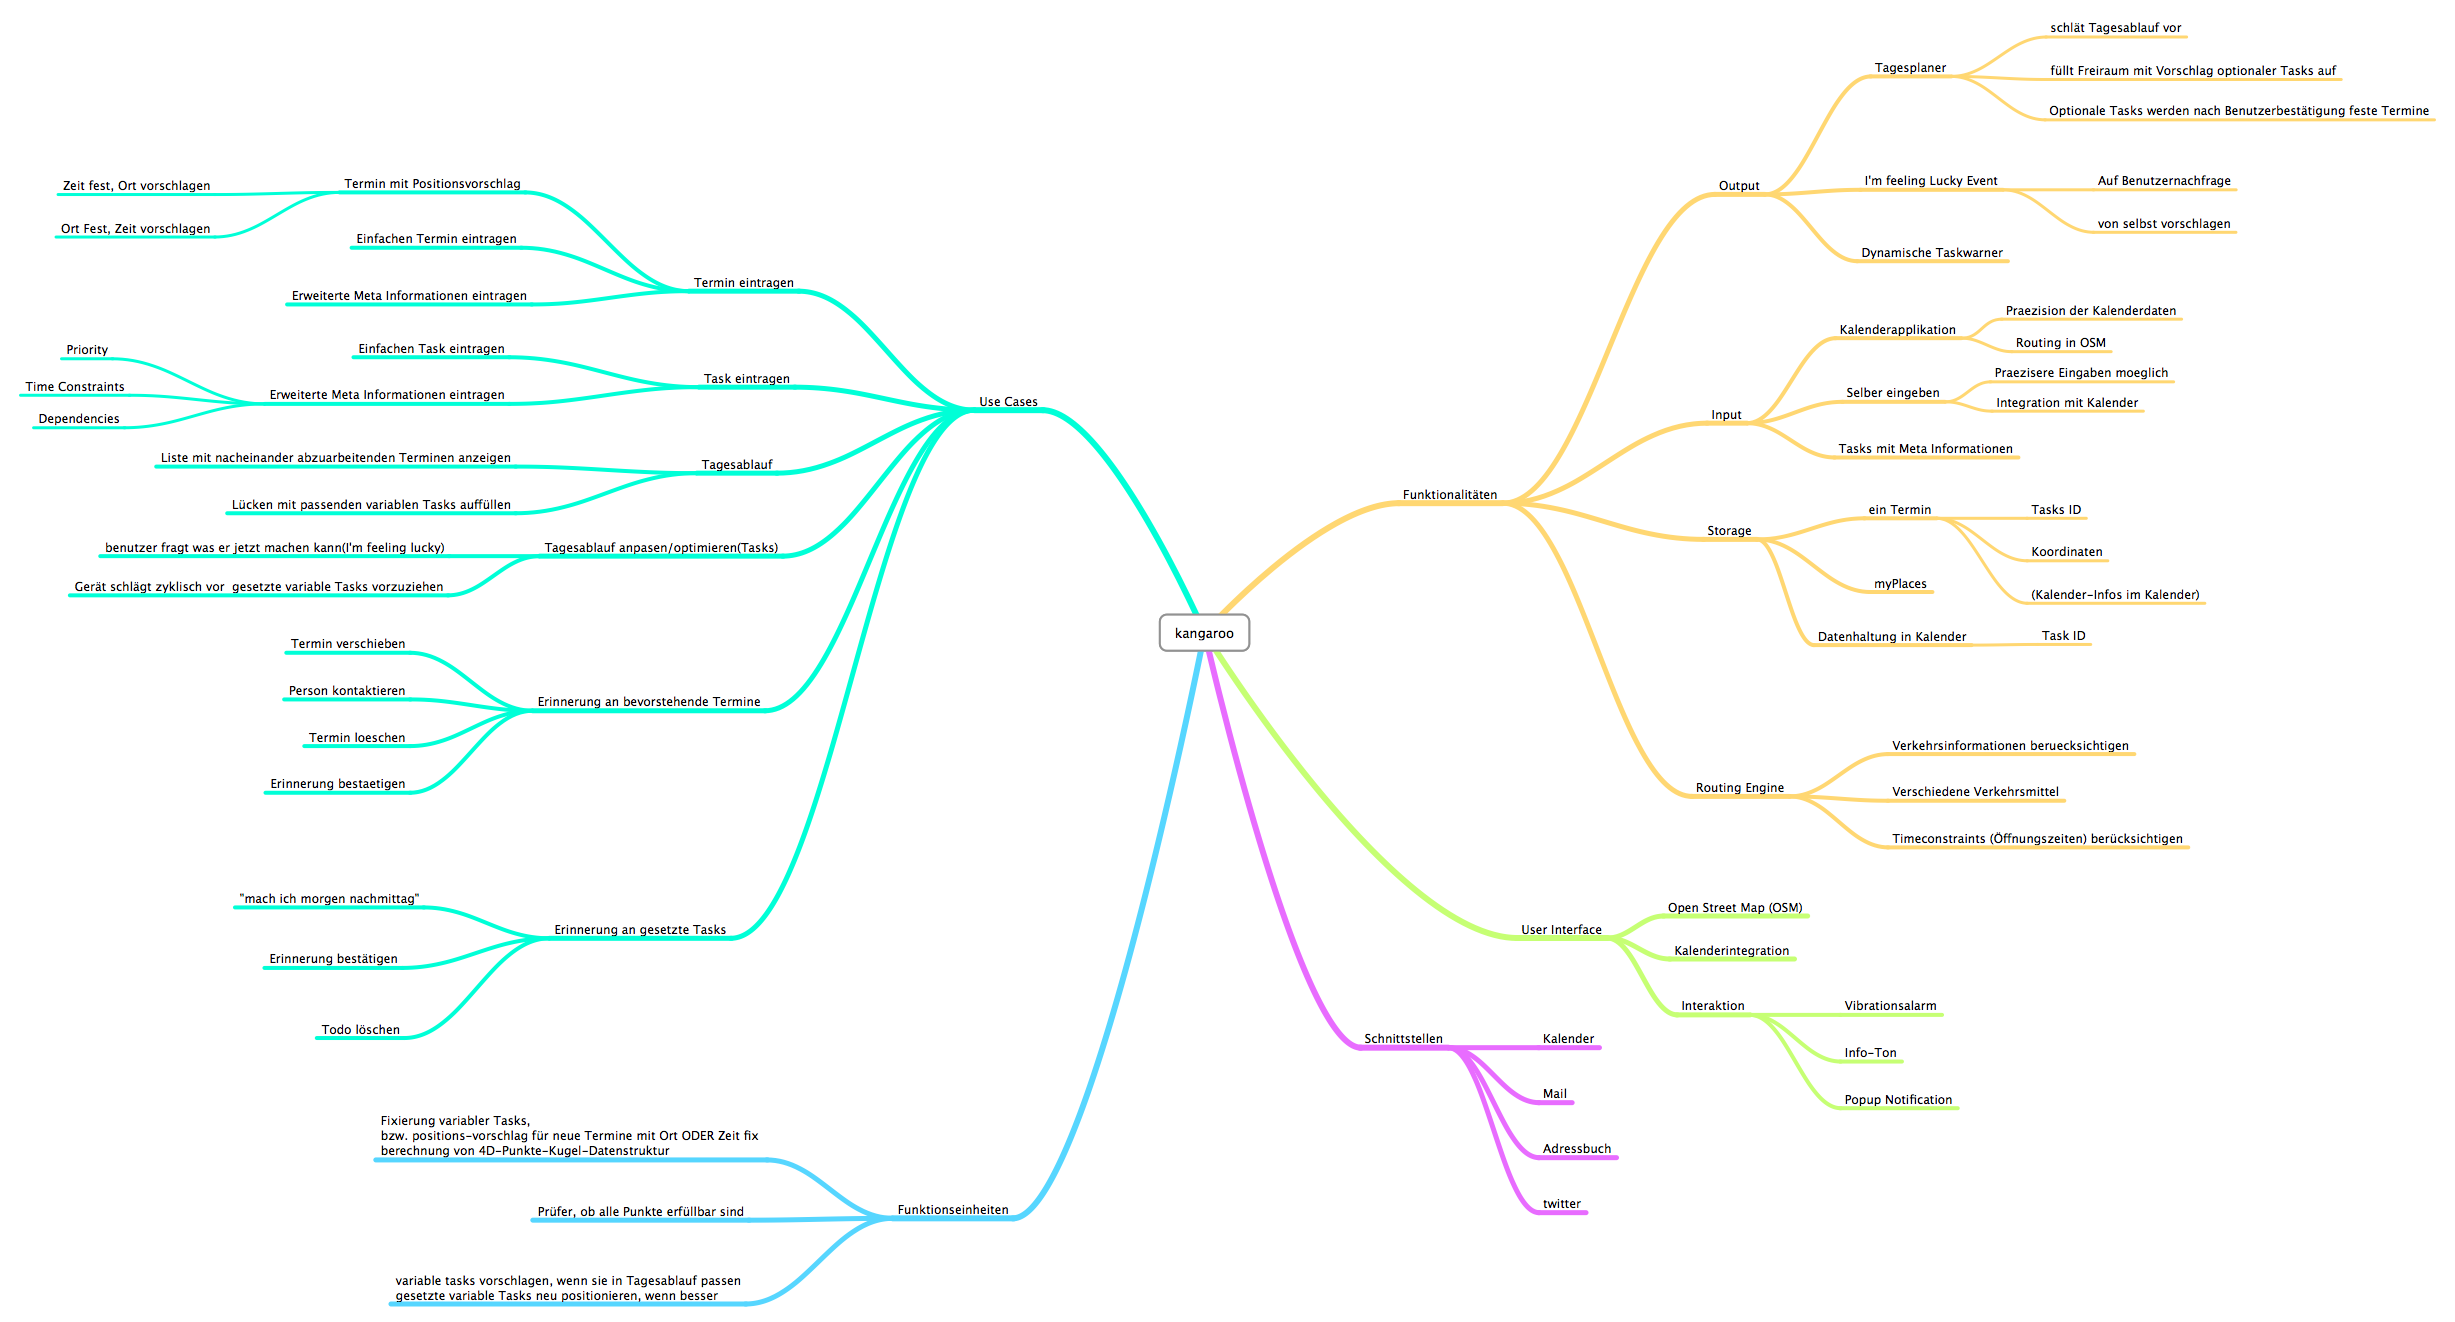
\includegraphics[width=16cm]{pics/kangaroo.png}
\caption{Mindmap with project goals, requirements and elements}
\label{mindmap}                                                                                                                                                  
\end{figure}
Based on the abstract requirements and the results of the brain-storming these development goals and principles ca be derived:
\begin{itemize}
\item The program should run on a mobile platform. At the moment several mobile operating systems are in use, competing for market shares. Since a consolidation of this market has not jet set in, the most appropriate platform for our use case has to be chosen.
\item For the application to be location aware, the mobile platform needs to provide access to location data from a GPS or a radio cell based location system.
\item The location awareness of the application is only then useful, when it is able to monitor its location continuous or in short intervals without interaction from the user and without disturbing the normal use of other applications. Therefore a part of the application needs to run in the form of a background process. This results in the requirements for the platform to support background execution of code and for the application to be highly energy efficient. A too high energy consumption by a continuous background task would drain the battery fast and render the whole application unusable.
\item For the location information to be helpful the application needs to be able to perform routing operation such as route finding, estimation of travel durations and localization of meaningful places. Since this is expected to be both complicated and with high computational complexity, an suitable existing routing solution needs to be found, evaluated and adapted. This is considered as one of the most critical requirements. 
\item To work with users dayplan, the application needs a way to handle tasks and appointments. In order to make the usage of as intuitive and easy as possible, the calendar and task-management functionality provided by the target platform shall be used.
\item In order to avoid the problem with digital traces and information leakage, the application shall run strictly local and shall be self sustained. This means all information that is used needs to be present on the device and all calculations need to be performed locally. No internet connection should be required for the application to function.
\item In order to make a re-usage of parts of the software or a further development of the application as a whole possible, the following properties need to be maintained during the development:
	\begin{itemize}
	\item a clean and adaptable system structure in order to enable the re-usage of single system parts in different projects
	\item a high level of code quality to minimize the time future developers need to adapt and learn to use the system.
	\item a detailed and well structured documentation to make future work with the code easier.
	\item only well-known and proven open-source tools and and software components shall be used that do not pose any problems in acquisition or usage for future developers.  
	\end{itemize}
\item In order to make a successful outcome of the project as likely as possible, a well-defined and formal project plan and development process shall be used. 
\end{itemize}
